\section*{Informations générales}
 
\begin{table}[H]
\centering
	\begin{tabularx}{16.8cm}{|X|X|}
	\hline
	\rowcolor{gray!40} Numéro du risque & Type du risque \\
	\hline
	007 &  Remise des données en avance \\
	\hline
	\end{tabularx}
\end{table}

\begin{table}[H]
\centering
	\begin{tabularx}{12.8cm}{|X|X|X|}
	\hline
	\rowcolor{gray!40} Date & Visa du \RQ & Visa du \CP \\
	\hline
	 29/01/2016 & pgpic & pgpic \\
	\hline
	\end{tabularx}
\end{table}

\begin{table}[H]
\centering
	\begin{tabularx}{12.8cm}{|X|X|X|X|}
	\hline
	\rowcolor{gray!40} Pilote & Activité WBS & Compte WBS & Phase d'apparition \\
	\hline
	 \Sergi & Suivre les Risques et Opportunités & 1.2.3.2 & Dès la demande auprès du client.\\
	\hline
	\end{tabularx}
\end{table}

\section*{Description du risque}

\subsection*{Résumé}
	La possibilité de recevoir les données du client en avance permettrait d'effectuer les tests et le remplissage de la base en avance.
	
\subsection*{Analyse des causes}
	voir figure.

\subsection*{Criticité}

\begin{table}[H]
\centering
	\begin{tabularx}{12.8cm}{|>{\columncolor{gray!40}}X|X|}
	\hline
	Bénéfice & 3\\
	\hline
	Probabilité & 3\\
	\hline
	Criticité & Moyen\\
	\hline
	\end{tabularx}
\end{table}
\newpage

\section*{Actions}
\subsection*{Actions proactives}

%\begin{table}[H]
\centering
	\begin{longtable}{|p{7cm}|p{7cm}|}
	\hline
	\rowcolor{gray!40} Nom de cause & Actions proactives \\
	\hline
	 Mise en place d'outils de communication adaptés & \begin{itemize}
	 	\item rechercher l'outil le plus performant
	 	\item se former sur les outils de communication
	 	\item demander aux anciens PICs le nom de leurs outils
	 \end{itemize} \\
	\hline
	Bonne planification & \begin{itemize}
		\item Bien former le \CP à la planification
		\item Etre présents et assidus
		\item Créneaux horaires respectés
		\item Objectifs personnels
	\end{itemize} \\
	\hline
	\end{longtable}
%\end{table}



\section*{Décision de clôture}
Par le \CP{} et le pilote du risque.
\begin{table}[H]
\centering
	\begin{tabularx}{12.8cm}{|X|X|}
	\hline
	\rowcolor{gray!40} Date de clôture & Raison de la clôture \\
	\hline
	  & \\
	\hline
	\end{tabularx}
\end{table}

\section*{Historique des modifications}
\begin{table}[H]
\centering
	\begin{tabularx}{12.8cm}{|X|X|}
	\hline
	Date & Modification \\
	\hline
	  & \\
	\hline
	\end{tabularx}
\end{table}
\newpage

\begin{figure}
	\centering
	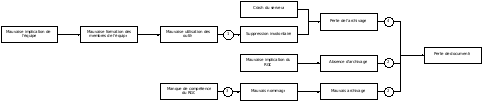
\includegraphics[scale=0.35]{images/AnalyseRisque_nPourquoi_FDR007}
\end{figure}